\section{Methodology}
\label{sec:methodology}
In our framework, we treat each consumer-item as an individual object and shape them into weekly time series data
based on historical transactions, where the target value at each time step (week) takes a binary input, 1/0 
(purchased/not purchased).
We apply sliding windows testing routine which is commonly referred to as walk-forward testing in order to generate 
out of time results. The time series is split into 4 parts - train, validation, 
test1, and test2 as shown in Table \ref{tab:datasplit}. All our models are built in a multi-object 
fashion, which allows the gradient movement to happen across all time series samples together. This also enables 
cross-learning to happen across time series and increases the number of training samples for model 
robustness. We then perform Feature Engineering over time series data to generate multiple types of features. 
Below are some of the feature groups we experimented with explicitly or unexplicitly:
\begin{itemize}
\item {\bf Datetime:} Transactional metrics at various temporal cuts including week, month and quarter. 
Datetime related features capturing seasonality and trend.
\item {\bf Consumer-Item Profile:} Transactional metrics at different granularities including consumer, item,
consumer-item, department, aisle, etc. The metrics includes some of likes Time since first order, 
Time since last order, time gap between orders, Reorder rates, Reorder frequency, 
Streak - user purchased the item in a row, Average position in the cart, Total number of orders.
\item {\bf Consumer-Item-Time Profile:} Transactional metrics at the intersection of consumer, item and time.
Interactions capturing consumer behaviour towards items for the given time period.
\end{itemize}
The model we needed to build, thus, should learn to identify similarly behaving time series across latent
parameters, and take into account consumer and item variations in comparing the time series. In our framework, a row 
in time series is represented by
  \begin{equation}
    \begin{array}{l}
      y\textsubscript{cit}  = f(i\textsubscript{t}, c\textsubscript{t},..,c\textsubscript{t-n}, ic\textsubscript{t}
      ,..,ic\textsubscript{t-n}, d\textsubscript{t},..,d\textsubscript{t-n})
    \end{array}
    \label{eqn:fx}
  \end{equation}
where y\textsubscript{cit} is purchase prediction for consumer 'c' item ’i’ at time ’t’. 
i\textsubscript{t} is attribute of the item ’i’ like category, department, brand, color, size, etc. 
c\textsubscript{t} is attribute of the consumer 'c' like age, sex and transactional attributes. 
ic\textsubscript{t} is transactional attributes of the consumer 'c'  towards item 'i'. 
d\textsubscript{t} is derived from datetime to capture trend and seasonality. 
Finally, n is the number of time lags.
\begin{table}[t]
\caption{Modelling data splits}
\vspace{0.1 in}
\centering
\resizebox{3.3in}{!}
{%
\begin{tabular}{|c|c|c|c|}
\hline
{\bf Data Split} & {\bf Specifications} & {\bf Consumer-Item combinations} & {\bf Max Time-Series length} \\  
\hline\hline
Train  		&  Model training &  50,872 &  46 weeks \\ \hline
Validation	  		&  Hyper-Parameter Optimization &  50,888 &  2 weeks \\ \hline
Test1  		&  Stacked Generalization, F\textsubscript{1}-Maximization & 50,899 &  2 weeks\\ \hline
Test2	  		&  Reporting Accuracy Metrics & 50,910 &  2 weeks\\
\hline
\end{tabular}
}
\label{tab:datasplit}
\end{table}
\subsection{Loss Function}
Since we are solving Binary classification problem, Binary Cross-Entropy/Log Loss seemed most logical loss function 
for training the models. Below is the formula to calculate Binary Cross-Entropy:
  \begin{equation}
      \begin{array}{l}
        H\textsubscript{p} = - \frac{1}{N}$$\sum_{i=1}^{N}y\textsubscript{i}.log(p(y\textsubscript{i}))+
        (1- y\textsubscript{i}).log(1-p(y\textsubscript{i}))
      \end{array}
    \label{eqn:logloss}
  \end{equation}
here H\textsubscript{p} represents computed loss, y\textsubscript{i} is the target value (label), and p(y\textsubscript{i}) 
is the predicted probability against the target. The value of BCELoss lies between 0 to 1. We can infer 
from Equation \ref{eqn:logloss} that Lower the BCELoss, better the Accuracy.
\subsection{Model Architectures}
As mentioned above, traditional machine learning models are not really a suitable choice for modelling \emph{f} 
Equation \ref{eqn:fx}. Hence, we work with machine learning tree based models like RandomForest, Xgboost \cite{chen2016xgboost} 
to Deep learning models ranging from Multi Layer Perceptron (MLP), Long Short 
Term Memory (LSTM) and Temporal Convolutional Networks (TCN). Architectures of MLP, LSTM, TCN \cite{lea2016temporal} 
and TCN-LSTM \cite{karim2017lstm} models are shown in Figure \ref{fig:MLP}, Figure \ref{fig:LSTM}, Figure \ref{fig:TCN}
and Figure \ref{fig:TCN-LSTM}, and have been explained below.
\begin{itemize}
\item {\bf Entity Embeddings + Multi Layer Perceptron:} : (MLP) Figure \ref{fig:MLP} is the simplest form of deep neural networks and was 
proposed in \cite{wang2017time} as a baseline architecture for Time Series classification. The architecture contains 
three hidden layers fully connected to the output of its previous layer. The final layer 
is the sigmoid layer to generate probabilities. One disadvantage is that since the input time 
series is fully connected to the first hidden layer, the temporal information in a time series is lost \cite{fawaz2019deep1}.
\item {\bf Entity Embeddings + Long Short Term Memory:} (LSTM) Figure \ref{fig:LSTM} is a sequence to sequence \cite{sutskever2014sequence} 
architecture comprising of 2 LSTM layers combined with entity embeddings. This combination flows into 
3 fully connected ReLU based layers yielding to dense layer which has sigmoid activation.
\item {\bf Entity Embeddings + Temporal Convolutional Network:} (TCN) Figure \ref{fig:TCN}, originally
proposed in \cite{lea2016temporal} , is considered a competitive architecture yielding the best results when evaluated over 
our experimental dataset. This network is comprised of 3 dilated Convolutional network combined with entity embeddings.
Similar to LSTM, it is also a sequence to sequence architecture which, after convolving and concatenation flows into 
3 fully connected ReLU based layers yielding to dense layer which has sigmoid activation.
\item {\bf Entity Embeddings + Long Short Term Memory-Temporal Convolutional Network:} (TCN-LSTM) Figure \ref{fig:TCN-LSTM} 
is again sequence to sequence architecture which inherits the properties of LSTM and TCN in a fully 
connected network.
\end{itemize}
As described in data classification Figure \ref{fig:dnndata}, the data was divided into following groups:
\begin{itemize}
\item {\bf Static Categorical:} These are categorical features which donot vary with time. This includes the consumer
attributes like sex, marital status and location, different item attributes like category, department and brand.
\item {\bf Temporal Categorical:} These are categorical features which vary with time. It includes all the datetime 
related features like week, month of year, etc.
\item {\bf Static Continuous:} These features are static but Continuous. This includes certain consumer attributes like
age and weight, item attributes like size, and certain derived features like target encoded features.
\item {\bf Temporal Continuous:} These are time varying Continuous features. All consumer and item related
traditional attributes like number of orders, add to cart order, etc. falls under this bucket.
\end{itemize}
As mentioned, in all the above described neural network architectures, we learn the embeddings \cite{guo2016entity} of the 
categorical features during training phase. We embed these attributes in order to both compress their representations 
while preserving salient features, and capture mutual similarities and differences.
  \begin{figure}[t]
    \centering 
    \caption{Data classification for DNN Architectures} 
    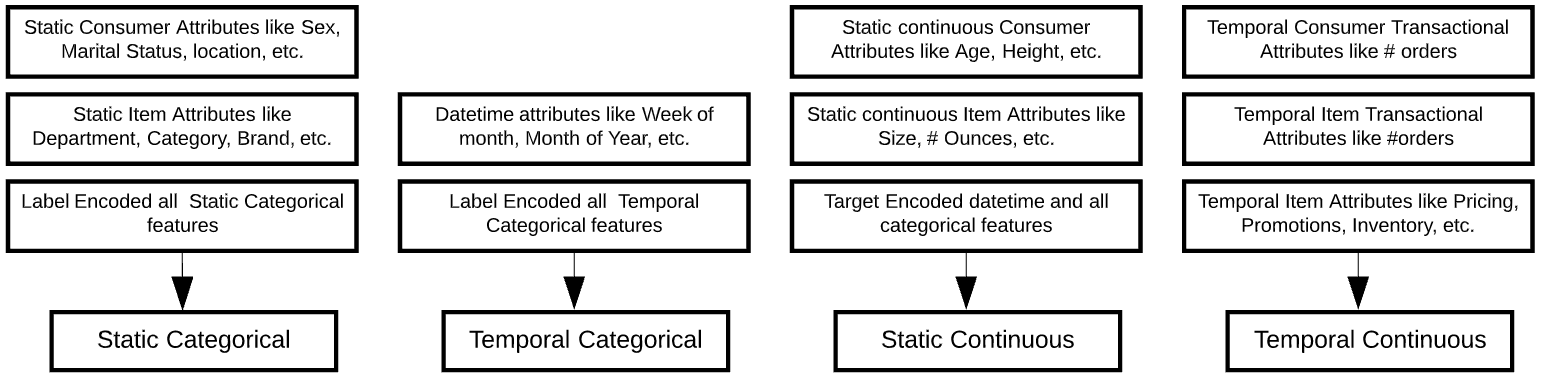
\includegraphics[width=3.3in]{img/dnndata.png} 
    \label{fig:dnndata} 
  \end{figure}
  \begin{figure}[t]
    \centering 
    \caption{Multi Layer Perceptron (MLP)} 
    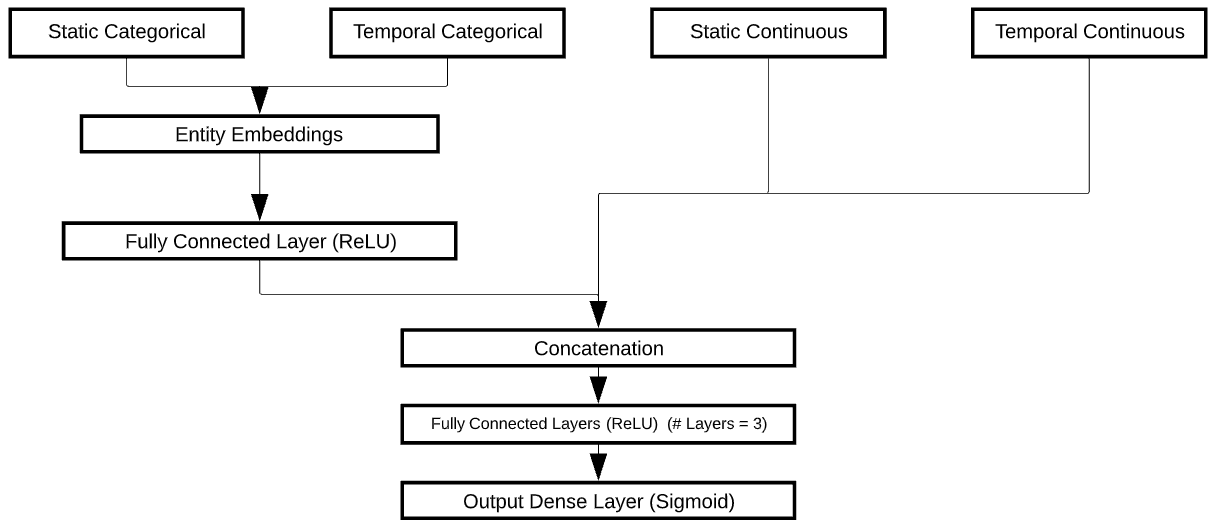
\includegraphics[width=3.3in]{img/MLP.png} 
    \label{fig:MLP} 
  \end{figure}
  \begin{figure}[t]
    \centering 
    \caption{Long Short Term Memory (LSTM)} 
    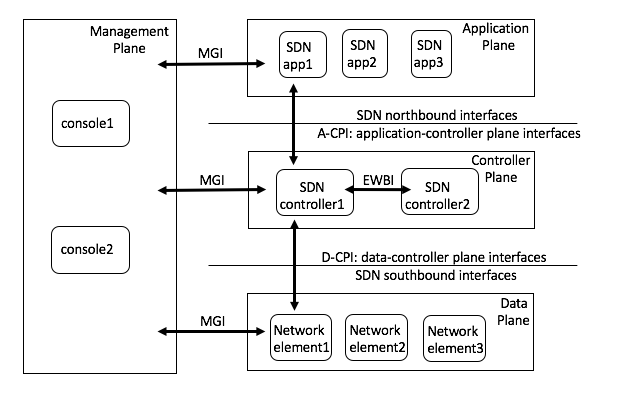
\includegraphics[width=3.3in]{img/LSTM.png} 
    \label{fig:LSTM} 
  \end{figure}
  \begin{figure}[t]
    \centering 
    \caption{Temporal Convolutional Network (TCN)} 
    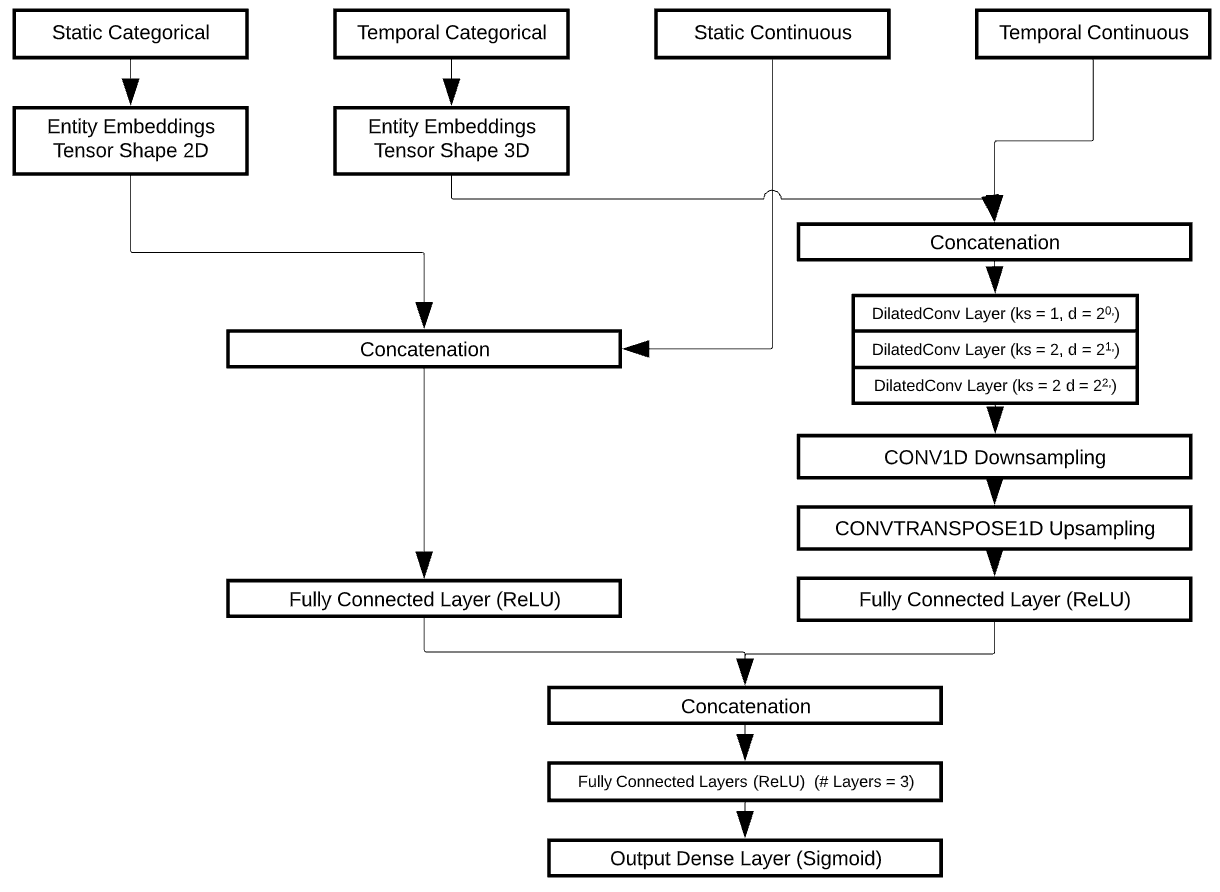
\includegraphics[width=3.3in]{img/TCN.png} 
    \label{fig:TCN} 
  \end{figure}
  \begin{figure}[t]
    \centering 
    \caption{TCN-LSTM} 
    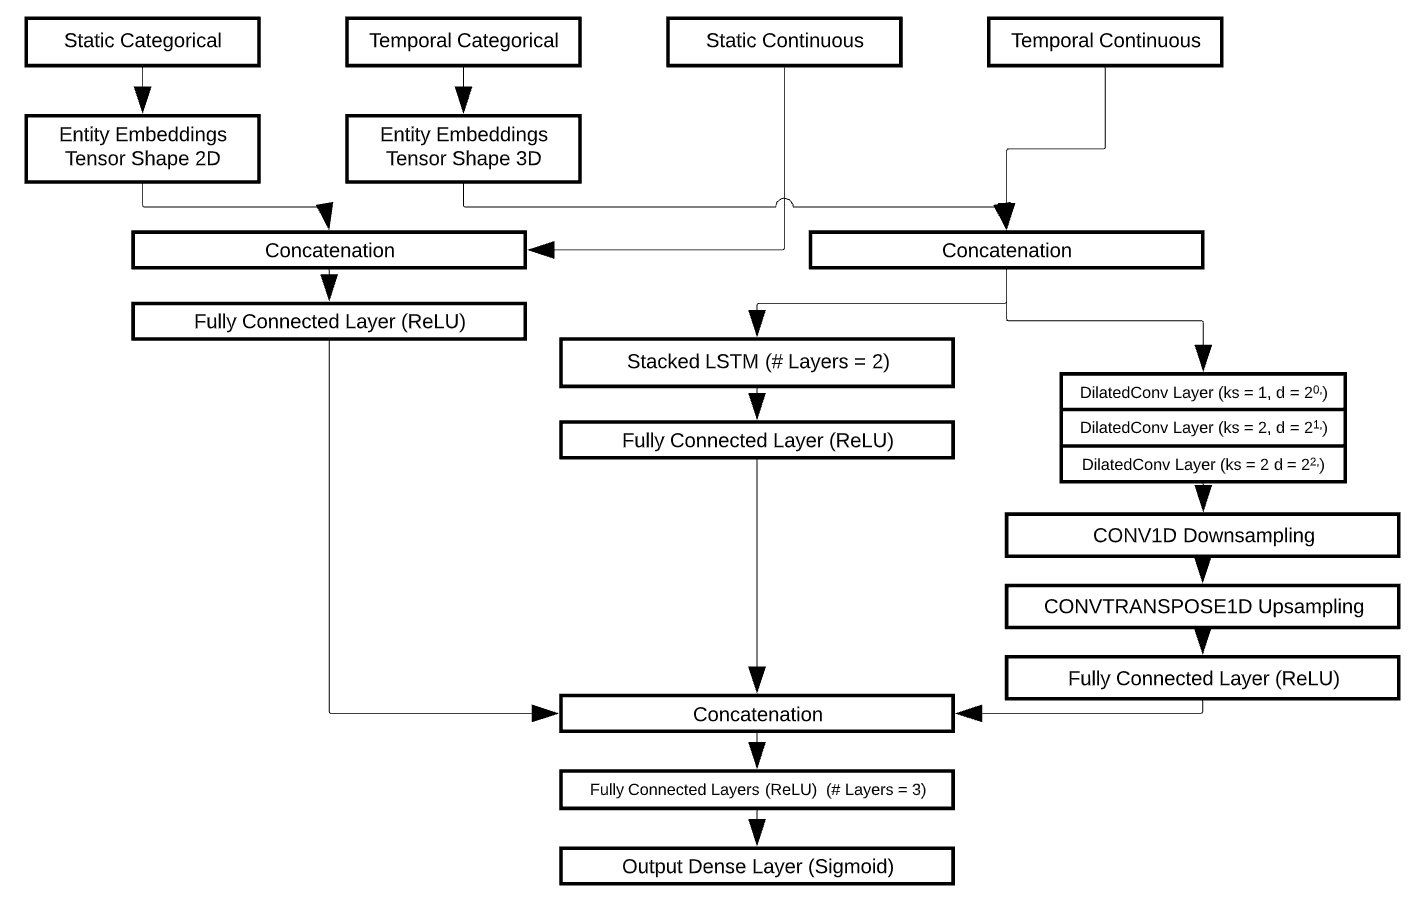
\includegraphics[width=3.3in]{img/TCNLSTM.png} 
    \label{fig:TCN-LSTM} 
  \end{figure}

The consumer purchase pattern has huge variation in terms of time of purchase (weekday/weekends), 
cadence of purchase (days to months), purchased item types (dairy/meat/grocery/apparels/etc.)
and brand loyalty (tendency to substitute items). Given such huge variance it becomes imperative 
to cross learn consumer behaviour from like consumer groups. To learn such relationships its very 
important to capture non-linear relationship between target and regressors at the most granular level.
Tree based and Deep learning models are chosen for their ability to model feature interactions even if transient in time, 
so that they capture non-linearity well. Utility of traditional machine learning algorithms like Logistic regression
, SVM and recommender systems are limited given the scale of large retail firms 
(Millions of customers with thousands of products). Such models do not scale well for large sets of data and hyperparameters.

Tree based models and MLP are trained in such a way where lagged values of time varying features are used
to capture temporal dependencies. LSTM, TCN and TCN-LSTM models are trained in sequence to sequence 
fashion \cite{sutskever2014sequence} using entire life-cycle data of a time series (Consumer-Item).
We use lagged values of temporal features for multiple time steps, lagged values combined with offsets in the form 
of statistical rolling operations like mean, median, quantiles, variance, 
kurtosis and skewness over varying lag periods are used for feature generation. More details around dataset and features 
are explained in section \ref{sec:eval}. 

\subsection{Hyperparameter Tuning}
Hyper-parameters of tree based models are optimized
using Bayesian Hyper-parameter Optimization Technique \cite{bergstra2013hyperopt}. We use documented best practices in deep 
learning along with some experiments and domain understanding to choose model hyperparameters like learning rate.
All hyperparameter Optimization was performed over Validation dataset. 
We list some of the params along with the values we used for Deep learning models.
  \begin{itemize}
    \item {\bf Optimizer Parameters:} RMSProp \cite{bengio2015rmsprop} and Adam were used as different trial configurations. The learning rate 
    was experimentally tuned to 1e-3. We also did weight decay of 1e-5 which helped a bit in model Regularization.
    \item {\bf Scheduler Parameters:} Cyclic \cite{smith2017cyclical} and ReduceLROnPlateau \cite{zaheer2018adaptive} 
    Learning rates were used as different trial configurations.
    we used 1e-3 as max lr and 1e-6 as base lr for Cyclical learning rate along with the step size being the function of
    length of train loader. ReduceLROnPlateau was tuned for 1e-6 as min lr.
    \item {\bf SWA:} Stochastic Weight Averaging (SWA) \cite{izmailov2018averaging} is used to improve generalization across Deep Learning
    models. SWA performs an equal average of the weights traversed by SGD with a modified learning rate schedule. We used 
    1e-3 as SWA learning rate.
    \item {\bf Parameter Average:} This applies weighted average over the parameter weights of n best performing epochs 
    (local minimas) from state dictionary post completion of training.
  \end{itemize}
Apart from the above parameters we also iterated enough to tune network parameters like number of epochs, batch size, 
number of Fully Connected Layers, number of LSTM layers, convnet parameters (kernel size, dilations, padding)
and embedding sizes for the categorical features. Binary Cross-Entropy/Log Loss \ref{eqn:logloss} was used as loss 
function for all the models. For the the sequence model \cite{sutskever2014sequence}, we also incorporated 
Dropout \cite{hinton2012improving} and BatchNorm \cite{santurkar2018does} as regularization parameters.

As mentioned above, we used Bayesian Hyper-parameter Optimization (Hyperopt) \cite{bergstra2013hyperopt} for hyper configuration 
tuning with 100 trials. Some of the hyperparameters we used for Machine learning models are :
  \begin{itemize}
    \item {\bf Learning Rate:} Range set to vary between 1e-2 to 5e-1. 
    \item {\bf Max Depth:} Range set from 2 to 12 at step of 1.
  \end{itemize}
Apart from these, Regularization parameters like Reg Lambda, Min Sample Leaf was also optimized for using Hyperopt.

Deep learning models are built using deep learning framework
PyTorch \cite{paszke2017automatic}, and are trained on GCP instance containing 6 CPUs and a single GPU. 
scikit-learn \cite{pedregosa2011scikit} is used for Tree
based models like RandomForest and Xgboost \cite{chen2016xgboost}. 
We built a total of 60 models, 12 different param configurations for each of 4 
Deep Learning models and 6 best trials for each of 2 Machine Learning models as shown in Table \ref{tab:modelparams}.
\subsection{Stacked Generalization Ensemble}
Stacked Generalization Ensemble or Stacking \cite{wolpert1992stacked} is a method used to combine predictions from 
different models algorithmically.
We used Weighted K-Best as Stacker model for combining k models (candidates) out of total 60 from Table \ref{tab:modelparams}. 
Test1 BCELoss was used as metric to compute weight for each of the 60 candidates. We iterated with different 
values of k ranging from 3 to 25. For Stacking, we computed Weighted Average of prediction
probabilities from k individual models for Train, Validation, Test1 and Test2 for each time steps.
Above phenomenon of stacking can be represented as:
  \begin{equation}
    \begin{array}{l}
      y\textsubscript{cit} =\sum_{j=1}^{k}w\textsubscript{j} \times p\textsubscript{cit\textsubscript{j}}
    \end{array}
    \label{eqn:stack}
  \end{equation}
where y\textsubscript{cit} is the stacked probability for consumer 'c' item ’i’ at time ’t’.
k represents the number of candidates shortlisted for stacking and p\textsubscript{cit\textsubscript{k}}
represents the prediction probability for consumer 'c' item ’i’ at time ’t’ by k\textsuperscript{th} model.
w\textsubscript{k} is the candidate weight of k\textsuperscript{th} model.

\subsection{F\textsubscript{1}-Maximization}
Post generation of the consumer-item probabilities, we optimize for the purchase cut-off probability based on 
probability distribution of a time step at consumer level using F\textsubscript{1}-Measure \cite{lipton2014optimal}. 
To illustrate above, lets say we generated purchase probabilities for 
n\textsubscript{i} items of b\textsubscript{i} actually purchased items for consumer c\textsubscript{i}.
Let Actual items purchased by consumer c\textsubscript{i} at a time step be [Ia\textsubscript{1}, Ia\textsubscript{2}
,.., Ia\textsubscript{b\textsubscript{i}}] whereas items for which the model generated probabilities for the 
consumer c\textsubscript{i} at that time step be [Ip\textsubscript{1}, Ip\textsubscript{2} ,.., 
Ip\textsubscript{n\textsubscript{i}}]. 
  \begin{equation}
    \begin{array}{l}
      A\textsubscript{c\textsubscript{i}} = [a\textsubscript{1}, a\textsubscript{2}, .., a\textsubscript{n\textsubscript{i}}] 
       \; \forall \; a\textsubscript{j} \in \; $\{0,1\}$
    \end{array}
    \label{eqn:A}
  \end{equation}
  \begin{equation}
    \begin{array}{l}
      P\textsubscript{c\textsubscript{i}} = [p\textsubscript{1}, p\textsubscript{2}, .., p\textsubscript{n\textsubscript{i}}]
      \; \forall \; p\textsubscript{j} \in \; [0,1]
    \end{array}
    \label{eqn:P}
  \end{equation}
A\textsubscript{c\textsubscript{i}} represents the actuals for consumer c\textsubscript{i}, with a\textsubscript{j} being 1/0 
(purchased/non purchased). P\textsubscript{c\textsubscript{i}} represents the predicted probabilities 
for consumer c\textsubscript{i} for respective item, with p\textsubscript{j} being probability value. 
As mentioned above n\textsubscript{i} is the total items model generated purchase probabilities for.
  \begin{equation}
    \begin{array}{l}
      D(Pr\textsubscript{c\textsubscript{i}}) : P\textsubscript{c\textsubscript{i}}\textsuperscript{1 x n\textsubscript{i}}
      \to P\textsuperscript{'}\textsubscript{c\textsubscript{i}}\textsuperscript{1 x n\textsubscript{i}}
      \;\; : p\textsuperscript{'}\textsubscript{j} = 
        \begin{cases}
          1 & p\textsubscript{j} \geq Pr\textsubscript{c\textsubscript{i}} \\
          0 & p\textsubscript{j} < Pr\textsubscript{c\textsubscript{i}} 
        \end{cases}
    \end{array}
    \label{eqn:Decision}
  \end{equation}
  \begin{equation}
    \begin{array}{l}
      P\textsuperscript{'}\textsubscript{c\textsubscript{i}} = [p\textsuperscript{'}\textsubscript{1}, 
      p\textsuperscript{'}\textsubscript{2}, .., p\textsuperscript{'}\textsubscript{n\textsubscript{i}}]\; 
      \forall \; p\textsuperscript{'}\textsubscript{j} \in \; $\{0,1\}$
    \end{array}
    \label{eqn:Pdash}
  \end{equation}
  \begin{equation}
    \begin{array}{l}
      k\textsubscript{i} =\sum_{i=1}^{n\textsubscript{i}}p\textsuperscript{'}\textsubscript{i}
    \end{array}
    \label{eqn:Pdash}
  \end{equation}
Pr\textsubscript{c\textsubscript{i}} is the probability cut-off to be optimized for consumer c\textsubscript{i}.
Decision rule D converts probabilities P\textsubscript{c\textsubscript{i}} to binary predictions 
P\textsuperscript{'}\textsubscript{c\textsubscript{i}} such that if p\textsubscript{j} is less than 
Pr\textsubscript{c\textsubscript{i}} then p\textsuperscript{'}\textsubscript{j} equals 0 else 1. 
k\textsubscript{i} is the total number of predictions which Decision rule D converted to 1 or in other words
number of predictions which model predicted as purchase.
  \begin{equation}
    \begin{array}{l}
      V\textsubscript{Pr\textsubscript{c\textsubscript{i}}} = 
      P\textsuperscript{'}\textsubscript{c\textsubscript{i}}
      \;\times\; A\textsubscript{c\textsubscript{i}}\textsuperscript{T}
      \;
      \Rightarrow	
      \left( \begin{array}{ccc}
      p\textsuperscript{'}\textsubscript{1} & .. & 
      p\textsuperscript{'}\textsubscript{n\textsubscript{i}}
      \end{array} \right)
      \times
      %
      \left( \begin{array}{ccc}
      a\textsubscript{1} \\
      .. \\
      a\textsubscript{n\textsubscript{i}} \\
      \end{array} \right)
    \end{array}
    \label{eqn:probability}
  \end{equation}
V\textsubscript{Pr\textsubscript{c\textsubscript{i}}} represents the number of items with purchase 
probabilities greater than Pr\textsubscript{c\textsubscript{i}} which were actually purchased (True Positives). 
Now using the below formulae we calculate Precision, Recall and F\textsubscript{1}-score for consumer c\textsubscript{i}.
  \begin{equation}
    \begin{array}{l}
      Precision\textsubscript{c\textsubscript{i}}= \frac{V\textsubscript{Pr\textsubscript{c\textsubscript{i}}}} {k\textsubscript{i}}
      \;\;\;\;\;and\;\;\;\;
      Recall\textsubscript{c\textsubscript{i}}= \frac{V\textsubscript{Pr\textsubscript{c\textsubscript{i}}}} {b\textsubscript{i}}
    \end{array}
    \label{eqn:F1}
  \end{equation}
  \begin{equation}
    \begin{array}{l}
      F\textsubscript{1\textsubscript{c\textsubscript{i}}} = \frac{2 \times Precision\textsubscript{c\textsubscript{i}} 
      \times Recall\textsubscript{c\textsubscript{i}}} 
      {Precision\textsubscript{c\textsubscript{i}} + Recall\textsubscript{c\textsubscript{i}}}
      \;
      \;\;\;\;\Rightarrow	\;\;\;\;
      2 * 
      \frac{
        V\textsubscript{Pr\textsubscript{c\textsubscript{i}}}
      }
      {
        k\textsubscript{i} + b\textsubscript{i}
      }
    \end{array}
    \label{eqn:Optimizer}
  \end{equation}
F\textsubscript{1\textsubscript{c\textsubscript{i}}} becomes the value to be maximised
at optimal Pr\textsubscript{c\textsubscript{i}} for consumer c\textsubscript{i}.
We solve the above Optimization function over test1 probability distribution 
at a consumer level to find optimal probability cut-off Pr\textsubscript{c\textsubscript{i}} . 
Final purchase predictions are based on the cut-off value generated at consumer level.
\begin{center}
\begin{table*}[!t]
\caption{Model Specifications}
\centering
\resizebox{\textwidth}{!}{\begin{tabular}{|r|l|r|r|}
  \hline
 {\bf Model Type} & {\bf Trials} & {\bf Model Hyper-Parameters} & {\bf Loss Functions}\\ 
 \hline\hline
MLP	  		&  12 & Optimizer, Scheduler, SWA, Parameter Averaging, Feature Groups, FC Layers & BCELoss\\ \hline
LSTM  		& 12 & Optimizer, Scheduler, SWA, Parameter Averaging, Feature Groups, FC Layers, LSTM Layers & BCELoss \\ \hline
TCN			& 12	& Optimizer, Scheduler, SWA, Parameter Averaging, Feature Groups, FC Layers, Convolution Parameters  & BCELoss\\ \hline
TCN-LSTM 		& 12	& Optimizer, Scheduler, SWA, Parameter Averaging, Feature Groups, FC Layers, LSTM, Convolution Parameters  & BCELoss\\ \hline
Xgboost 		& 6	& Learning rate, Tree Depth, Regularization parameters  & BCELoss\\ \hline
RandomForest 		& 6	& Tree Depth, Evaluation Metrics, Regularization parameters &  BCELoss\\
   \hline
\end{tabular}}
\label{tab:modelparams}
\end{table*} 
\end{center}
